% Chapter 3: Seminar - ARIMA Models
% Harvard-quality academic presentation
% Bachelor program, Bucharest University of Economic Studies

\documentclass[9pt, aspectratio=169, t]{beamer}

% Ensure content fits on slides
\setbeamersize{text margin left=8mm, text margin right=8mm}

%=============================================================================
% THEME AND STYLE CONFIGURATION
%=============================================================================
\usetheme{default}
% Using default theme for clean header/footer control

% Color Palette (matching Redispatch PDF)
\definecolor{MainBlue}{RGB}{26, 58, 110}
\definecolor{AccentBlue}{RGB}{26, 58, 110}
\definecolor{IDAred}{RGB}{205, 0, 0}
\definecolor{DarkGray}{RGB}{51, 51, 51}
\definecolor{MediumGray}{RGB}{128, 128, 128}
\definecolor{LightGray}{RGB}{248, 248, 248}
\definecolor{VeryLightGray}{RGB}{235, 235, 235}
\definecolor{KeynoteGray}{RGB}{218, 218, 218}
\definecolor{SectionGray}{RGB}{120, 120, 120}
\definecolor{FooterGray}{RGB}{100, 100, 100}
\definecolor{Crimson}{RGB}{220, 53, 69}
\definecolor{Forest}{RGB}{46, 125, 50}
\definecolor{Amber}{RGB}{181, 133, 63}
\definecolor{Orange}{RGB}{230, 126, 34}
\definecolor{Purple}{RGB}{142, 68, 173}

% Gradient background (exact Keynote 315° gradient: white to RGB 218,218,218)
\setbeamertemplate{background}{%
    \begin{tikzpicture}[remember picture, overlay]
        \shade[shading=axis, shading angle=315,
        top color=white, bottom color=KeynoteGray]
        (current page.south west) rectangle (current page.north east);
    \end{tikzpicture}%
}
% Fallback solid color for compatibility
\setbeamercolor{background canvas}{bg=}

\setbeamercolor{palette primary}{bg=MainBlue, fg=white}
\setbeamercolor{palette secondary}{bg=MainBlue!85, fg=white}
\setbeamercolor{palette tertiary}{bg=MainBlue!70, fg=white}
\setbeamercolor{structure}{fg=MainBlue}
\setbeamercolor{title}{fg=IDAred}
\setbeamercolor{frametitle}{fg=IDAred, bg=}
\setbeamercolor{block title}{bg=MainBlue, fg=white}
\setbeamercolor{block body}{bg=VeryLightGray, fg=DarkGray}
\setbeamercolor{block title alerted}{bg=Crimson, fg=white}
\setbeamercolor{block body alerted}{bg=Crimson!8, fg=DarkGray}
\setbeamercolor{block title example}{bg=Forest, fg=white}
\setbeamercolor{block body example}{bg=Forest!8, fg=DarkGray}
\setbeamercolor{item}{fg=MainBlue}

% Footer colors (override Madrid theme blue)
\setbeamercolor{author in head/foot}{fg=FooterGray, bg=}
\setbeamercolor{title in head/foot}{fg=FooterGray, bg=}
\setbeamercolor{date in head/foot}{fg=FooterGray, bg=}
\setbeamercolor{section in head/foot}{fg=FooterGray, bg=}
\setbeamercolor{subsection in head/foot}{fg=FooterGray, bg=}

% Bullet styles (apply everywhere including blocks)
\setbeamertemplate{itemize item}{\color{MainBlue}$\boxdot$}
\setbeamertemplate{itemize subitem}{\color{MainBlue}$\blacktriangleright$}
\setbeamertemplate{itemize subsubitem}{\color{MainBlue}\tiny$\bullet$}
\setbeamertemplate{itemize/enumerate body begin}{\normalsize}
\setbeamertemplate{itemize/enumerate subbody begin}{\normalsize}

% Item spacing - compact style
\setlength{\leftmargini}{10pt}       % Level 1: minimal indent
\setlength{\leftmarginii}{10pt}      % Level 2: minimal additional indent
% Compact list spacing (zero extra space before/after lists in blocks)
\makeatletter
\def\@listi{\leftmargin\leftmargini \topsep 0pt \parsep 0pt \itemsep 0pt}
\def\@listii{\leftmargin\leftmarginii \topsep 0pt \parsep 0pt \itemsep 0pt}
\makeatother

\setbeamertemplate{navigation symbols}{}

%=============================================================================
% CUSTOM HEADLINE
%=============================================================================
\setbeamertemplate{headline}{%
    \vskip10pt%
    \hbox to \paperwidth{%
        \hskip0.5cm%
        {\small\color{FooterGray}\renewcommand{\hyperlink}[2]{##2}\insertsectionhead}%
        \hfill%
        \textcolor{FooterGray}{\small\insertframenumber}%
        \hskip0.5cm%
    }%
    \vskip4pt%
    {\color{FooterGray}\hrule height 0.4pt}%
}

%=============================================================================
% CUSTOM FOOTER
%=============================================================================
\usepackage{fontawesome5}

\setbeamertemplate{footline}{%
    {\color{FooterGray}\hrule height 0.4pt}%
    \vskip4pt%
    \hbox to \paperwidth{%
        \hskip0.5cm%
        \textcolor{FooterGray}{\small Time Series Analysis and Forecasting}%
        \hfill%
        \raisebox{-0.1em}{%
            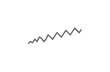
\begin{tikzpicture}[x=0.08em, y=0.08em, line width=0.4pt]
                \draw[FooterGray] (0,3) -- (1,4) -- (2,3.5) -- (3,5) -- (4,4) -- (5,6) -- (6,5.5) -- (7,4) -- (8,5) -- (9,7) -- (10,6) -- (11,5) -- (12,6.5) -- (13,8) -- (14,7) -- (15,6) -- (16,7.5) -- (17,9) -- (18,8) -- (19,7) -- (20,8.5) -- (21,10) -- (22,9) -- (23,8) -- (24,9.5);
            \end{tikzpicture}%
        }%
        \hskip0.5cm%
    }%
    \vskip6pt%
}

%=============================================================================
% PACKAGES
%=============================================================================
\usepackage[utf8]{inputenc}
\usepackage[T1]{fontenc}
\usepackage[english]{babel}
\usepackage{amsmath, amssymb, amsthm}
\usepackage{mathtools}
\usepackage{bm}
\usepackage{tikz}
\usetikzlibrary{arrows.meta, positioning, shapes, calc, decorations.pathreplacing, shadings}
\usepackage{booktabs}
\usepackage{multirow}
\usepackage{array}
\usepackage{graphicx}
\usepackage{hyperref}
\usepackage{colortbl}
\hypersetup{colorlinks=true, linkcolor=MainBlue, urlcolor=MainBlue}
\graphicspath{{../../logos/}{../../charts/}}
\hfuzz=2pt  % Suppress tiny overfull warnings (<2pt)
\vfuzz=2pt  % Suppress tiny vertical overfull warnings (<2pt)

%=============================================================================
% QUANTLET COMMAND
%=============================================================================
\newcommand{\quantlet}[2]{%
    \hfill\href{#2}{%
        \raisebox{-0.15em}{\includegraphics[height=0.7em]{ql_logo.png}}%
        \textcolor{MainBlue}{\tiny\ #1}%
    }%
}

%=============================================================================
% THEOREM ENVIRONMENTS
%=============================================================================
\theoremstyle{definition}
\setbeamertemplate{theorems}[numbered]
\newtheorem{defn}{Definition}
\newtheorem{thm}{Theorem}
\newtheorem{prop}{Proposition}
\newtheorem{rmk}{Remark}

%=============================================================================
% CUSTOM COMMANDS
%=============================================================================
\newcommand{\E}{\mathbb{E}}
\newcommand{\Var}{\text{Var}}
\newcommand{\Cov}{\text{Cov}}
\newcommand{\Corr}{\text{Corr}}
\newcommand{\R}{\mathbb{R}}
\newcommand{\N}{\mathbb{N}}
\newcommand{\Z}{\mathbb{Z}}
\newcommand{\RMSE}{\text{RMSE}}
\newcommand{\MAE}{\text{MAE}}
\newcommand{\MAPE}{\text{MAPE}}

% Quiz styling
\newcommand{\correct}{\textcolor{Forest}{\checkmark}}
\newcommand{\incorrect}{\textcolor{Crimson}{\texttimes}}

%=============================================================================
% CUSTOM TITLE PAGE
%=============================================================================
\defbeamertemplate*{title page}{hybrid}[1][]
{
    \vspace{0.2cm}
    % Logos row - top header (with clickable links)
    \begin{center}
        \href{https://www.ase.ro}{\includegraphics[height=1.0cm]{ase_logo.png}}\hspace{0.3cm}%
        \href{https://theida.net}{\includegraphics[height=1.0cm]{ida_logo.png}}\hspace{0.3cm}%
        \href{https://blockchain-research-center.com}{\includegraphics[height=1.0cm]{brc_logo.png}}\hspace{0.3cm}%
        \href{https://www.ai4efin.ase.ro}{\includegraphics[height=1.0cm]{ai4efin_logo.png}}\hspace{0.3cm}%
        \href{https://ipe.ro/new}{\includegraphics[height=1.0cm]{acad_logo.png}}\hspace{0.3cm}%
        \href{https://www.digital-finance-msca.com}{\includegraphics[height=1.0cm]{msca_logo.png}}%
    \end{center}

    \vspace{0.6cm}

    % Main title with Q logos on sides (with clickable links)
    \begin{center}
        \begin{minipage}{0.1\textwidth}
            \centering
            \href{https://quantlet.com}{\includegraphics[height=1.1cm]{ql_logo.png}}
        \end{minipage}%
        \begin{minipage}{0.78\textwidth}
            \centering
            {\LARGE\bfseries\usebeamercolor[fg]{title}\inserttitle}

            \vspace{0.3cm}

            {\usebeamerfont{subtitle}\usebeamercolor[fg]{title}\insertsubtitle}
        \end{minipage}%
        \begin{minipage}{0.1\textwidth}
            \centering
            \href{https://quantinar.com}{\includegraphics[height=1.1cm]{qr_logo.png}}
        \end{minipage}
    \end{center}

    \vspace{0.6cm}

    % Authors (left aligned)
    \hspace{0.5cm}{\usebeamerfont{author}\insertauthor}

    \vspace{0.3cm}

    % Institute/Affiliations (left aligned)
    \hspace{0.5cm}\begin{minipage}[t]{0.9\textwidth}
        \raggedright\small\insertinstitute
    \end{minipage}
}

%=============================================================================
% TITLE INFORMATION
%=============================================================================
\title[Time Series Analysis]{Time Series Analysis and Forecasting}
\subtitle{Seminar 3: ARIMA Models}
\author[D.T. Pele]{Daniel Traian PELE}
\institute{Bucharest University of Economic Studies\\
IDA Institute Digital Assets\\
Blockchain Research Center\\
AI4EFin -- Artificial Intelligence for Energy Finance\\
Romanian Academy, Institute for Economic Forecasting\\
MSCA Digital Finance}
\date{}

\begin{document}

% Title page (no header/footer)
{
\setbeamertemplate{headline}{}
\setbeamertemplate{footline}{}
\begin{frame}
    \titlepage
\end{frame}
}

%=============================================================================
% SEMINAR OUTLINE
%=============================================================================
\section{Overview}

\begin{frame}{Seminar Outline}
    \textbf{\large Today's Activities:}

    \vspace{0.4cm}

    \begin{enumerate}
        \item[\textcolor{MainBlue}{\textbf{1.}}] \textbf{Review Quiz} --- Checking understanding of ARIMA concepts
        \vspace{0.15cm}
        \item[\textcolor{MainBlue}{\textbf{2.}}] \textbf{True/False Questions} --- Conceptual checks
        \vspace{0.15cm}
        \item[\textcolor{MainBlue}{\textbf{3.}}] \textbf{Practice Problems} --- Calculations with ARIMA
        \vspace{0.15cm}
        \item[\textcolor{MainBlue}{\textbf{4.}}] \textbf{Worked Examples} --- Real-world applications
        \vspace{0.15cm}
        \item[\textcolor{MainBlue}{\textbf{5.}}] \textbf{Discussion Questions} --- Practical applications
        \vspace{0.15cm}
        \item[\textcolor{MainBlue}{\textbf{6.}}] \textbf{AI-Assisted Exercises} --- Human vs.\ AI modeling
    \end{enumerate}
\end{frame}

%=============================================================================
% SECTION 1: REVIEW QUIZ
%=============================================================================
\section{Review Quiz}

\begin{frame}{Quiz 1: Integration Order}
    \begin{alertblock}{Question}
        A time series $Y_t$ requires two differences to become stationary. What is its order of integration?
    \end{alertblock}
    \vspace{0.1cm}

    \only<1>{
    \begin{enumerate}[A)]
        \item $I(0)$
        \item $I(1)$
        \item $I(2)$
        \item Cannot be determined
    \end{enumerate}
    }
    \only<2>{
    \begin{exampleblock}{Answer: C -- $I(2)$}
        \textbf{Definition}: $Y_t \sim I(d)$ if $\Delta^d Y_t$ is stationary but $\Delta^{d-1} Y_t$ is not.

        \textbf{Example}: If $Y_t$ follows $\Delta^2 Y_t = \varepsilon_t$, then:
        \begin{itemize}
            \item $\Delta Y_t = \Delta Y_{t-1} + \varepsilon_t$ (still has unit root)
            \item $\Delta^2 Y_t = \varepsilon_t$ (white noise, stationary)
        \end{itemize}

        \textbf{Real-world}: Price levels may be $I(2)$ when inflation itself is non-stationary.
    \end{exampleblock}
    }
\end{frame}

\begin{frame}{Visual: Integrated Processes}
    \begin{center}
        \includegraphics[width=0.95\textwidth]{ch3_def_integrated.pdf}
    \end{center}
    \vspace{-0.2cm}
    \small $I(0)$: stationary. $I(1)$: one difference needed. $I(2)$: two differences needed to become stationary.
    \quantlet{TSA\_ch3\_def\_integrated}{https://github.com/QuantLet/TSA/tree/main/TSA_ch3/TSA_ch3_def_integrated}
\end{frame}

\begin{frame}{Quiz 2: Random Walk Properties}
    \begin{alertblock}{Question}
        For a random walk $Y_t = Y_{t-1} + \varepsilon_t$ with $\Var(\varepsilon_t) = \sigma^2$, what is $\Var(Y_t)$?
    \end{alertblock}
    \vspace{0.05cm}
    \only<1>{
    \begin{enumerate}[A)]
        \item $\sigma^2$
        \item $t \cdot \sigma^2$
        \item $\sigma^2 / t$
        \item $\sigma^2 / (1-\phi^2)$
    \end{enumerate}
    }
    \only<2>{
    \begin{exampleblock}{Answer: B -- $t \cdot \sigma^2$}
        \vspace{-0.3cm}
        \begin{center}
            \includegraphics[width=0.75\textwidth, height=0.35\textheight, keepaspectratio]{sem3_rw_variance.pdf}
        \end{center}
        \vspace{-0.3cm}
        {\footnotesize
        \textbf{Proof}: $Y_t = \sum_{i=1}^{t}\varepsilon_i \Rightarrow \Var(Y_t) = t\sigma^2$ (grows linearly $\Rightarrow$ non-stationary!)
        }
    \end{exampleblock}
    }
    \quantlet{TSA\_ch3\_rw\_variance}{https://github.com/QuantLet/TSA/tree/main/TSA_ch3/TSA_ch3_rw_variance}
\end{frame}

\begin{frame}{Quiz 3: ADF Test Hypotheses}
    \begin{alertblock}{Question}
        In the Augmented Dickey-Fuller test, what is the null hypothesis?
    \end{alertblock}
    \vspace{0.1cm}

    \only<1>{
    \begin{enumerate}[A)]
        \item The series is stationary
        \item The series has a unit root
        \item The series has no autocorrelation
        \item The series is normally distributed
    \end{enumerate}
    }
    \only<2>{
    \begin{exampleblock}{Answer: B -- The series has a unit root}
        \textbf{ADF regression}: $\Delta Y_t = \alpha + \gamma Y_{t-1} + \sum_{j=1}^{p}\delta_j \Delta Y_{t-j} + \varepsilon_t$

        \textbf{Hypotheses}:
        \begin{itemize}
            \item $H_0: \gamma = 0$ (unit root, non-stationary)
            \item $H_1: \gamma < 0$ (stationary)
        \end{itemize}

        \textbf{Decision}: Reject $H_0$ if $t$-statistic $<$ critical value (e.g., $-2.86$ at 5\%)

        \textbf{Note}: Uses special Dickey-Fuller distribution, not standard $t$.
    \end{exampleblock}
    }
\end{frame}

\begin{frame}{Visual: ADF Test}
    \begin{center}
        \includegraphics[width=0.95\textwidth]{ch3_def_adf.pdf}
    \end{center}
    \vspace{-0.2cm}
    \small Left: stationary -- ADF rejects unit root. Right: non-stationary -- ADF fails to reject.
    \quantlet{TSA\_ch3\_def\_adf}{https://github.com/QuantLet/TSA/tree/main/TSA_ch3/TSA_ch3_def_adf}
\end{frame}

\begin{frame}{Quiz 4: ARIMA Notation}
    \begin{alertblock}{Question}
        What does ARIMA(2,1,1) mean?
    \end{alertblock}
    \vspace{0.1cm}

    \only<1>{
    \begin{enumerate}[A)]
        \item AR(2) on differenced data with MA(1) errors
        \item AR(1) with 2 differences and MA(1)
        \item MA(2) with 1 difference and AR(1)
        \item 2 lags, 1 trend, 1 seasonal component
    \end{enumerate}
    }
    \only<2>{
    \begin{exampleblock}{Answer: A -- AR(2) on differenced data with MA(1) errors}
        \textbf{ARIMA($p,d,q$)}: $\phi(L)(1-L)^d Y_t = \theta(L)\varepsilon_t$

        \textbf{ARIMA(2,1,1) expands to}:
        \[
        (1-\phi_1 L - \phi_2 L^2)(1-L)Y_t = (1+\theta_1 L)\varepsilon_t
        \]
        Or equivalently: $(1-\phi_1 L - \phi_2 L^2)\Delta Y_t = (1+\theta_1 L)\varepsilon_t$

        \textbf{Interpretation}: First difference the series, then fit ARMA(2,1) to $\Delta Y_t$.
    \end{exampleblock}
    }
\end{frame}

\begin{frame}{Visual: ARIMA Process}
    \begin{center}
        \includegraphics[width=0.90\textwidth, height=0.75\textheight, keepaspectratio]{ch3_def_arima.pdf}
    \end{center}
    \vspace{-0.3cm}
    {\small Top: original ARIMA series. Bottom: after differencing, use ACF/PACF to identify AR and MA orders.}
    \quantlet{TSA\_ch3\_def\_arima}{https://github.com/QuantLet/TSA/tree/main/TSA_ch3/TSA_ch3_def_arima}
\end{frame}

\begin{frame}{Quiz 5: Difference Operator}
    \begin{alertblock}{Question}
        What is $(1-L)^2 Y_t$ expanded?
    \end{alertblock}
    \vspace{0.2cm}
    \only<1>{
    \begin{enumerate}[A)]
        \item $Y_t - Y_{t-1}$
        \item $Y_t - 2Y_{t-1} + Y_{t-2}$
        \item $Y_t + 2Y_{t-1} + Y_{t-2}$
        \item $Y_t - Y_{t-2}$
    \end{enumerate}
    }
    \only<2>{
    \begin{exampleblock}{Answer: B -- $Y_t - 2Y_{t-1} + Y_{t-2}$}
        \textbf{Binomial expansion}: $(1-L)^2 = 1 - 2L + L^2$

        \textbf{Applied}: $(1-L)^2 Y_t = Y_t - 2Y_{t-1} + Y_{t-2}$ (the ``change in changes'')
    \end{exampleblock}
    }
\end{frame}

\begin{frame}{Quiz 6: KPSS vs ADF}
    \begin{alertblock}{Question}
        How does the KPSS test differ from the ADF test?
    \end{alertblock}
    \vspace{0.05cm}
    \only<1>{
    \begin{enumerate}[A)]
        \item KPSS tests for seasonality, ADF tests for trends
        \item KPSS has stationarity as null, ADF has unit root as null
        \item KPSS is more powerful than ADF
        \item There is no difference
    \end{enumerate}
    }
    \only<2>{
    \begin{exampleblock}{Answer: B -- Reversed null hypotheses}
        \vspace{-0.3cm}
        \begin{center}
            \includegraphics[width=0.68\textwidth, height=0.37\textheight, keepaspectratio]{sem3_adf_kpss.pdf}
        \end{center}
        \vspace{-0.3cm}
        {\footnotesize
        \textbf{Strategy}: Use both tests together for robust inference!
        }
    \end{exampleblock}
    }
    \quantlet{TSA\_ch3\_adf\_kpss}{https://github.com/QuantLet/TSA/tree/main/TSA_ch3/TSA_ch3_adf_kpss}
\end{frame}

\begin{frame}{Quiz 7: Overdifferencing}
    \begin{alertblock}{Question}
        If $Y_t \sim I(1)$ and we compute $\Delta^2 Y_t$, what happens?
    \end{alertblock}
    \vspace{0.05cm}
    \only<1>{
    \begin{enumerate}[A)]
        \item We get a better stationary series
        \item We introduce artificial negative autocorrelation
        \item The variance decreases
        \item Nothing changes
    \end{enumerate}
    }
    \only<2>{
    \begin{exampleblock}{Answer: B -- Artificial negative autocorrelation}
        \vspace{-0.3cm}
        \begin{center}
            \includegraphics[width=0.78\textwidth, height=0.36\textheight, keepaspectratio]{sem3_overdifferencing.pdf}
        \end{center}
        \vspace{-0.3cm}
        {\footnotesize
        \textbf{Diagnostic}: ACF at lag 1 $\approx -0.5$ signals overdifferencing. Reduce $d$ by 1!
        }
    \end{exampleblock}
    }
    \quantlet{TSA\_ch3\_overdifferencing}{https://github.com/QuantLet/TSA/tree/main/TSA_ch3/TSA_ch3_overdifferencing}
\end{frame}

\begin{frame}{Quiz 8: Forecast Variance}
    \begin{alertblock}{Question}
        For an ARIMA(0,1,0) model (random walk), how does forecast variance behave as horizon $h$ increases?
    \end{alertblock}
    \vspace{0.1cm}

    \only<1>{
    \begin{enumerate}[A)]
        \item Stays constant
        \item Decreases to zero
        \item Grows linearly with $h$
        \item Converges to a finite limit
    \end{enumerate}
    }
    \only<2>{
    \begin{exampleblock}{Answer: C -- Grows linearly with $h$}
        \textbf{Random walk forecast}: $\hat{Y}_{T+h|T} = Y_T$ (best forecast is current value)

        \textbf{Forecast error}: $Y_{T+h} - \hat{Y}_{T+h|T} = \sum_{i=1}^{h} \varepsilon_{T+i}$

        \textbf{Variance}:
        \[
        \Var(Y_{T+h} - \hat{Y}_{T+h|T}) = h\sigma^2
        \]

        \textbf{95\% CI}: $Y_T \pm 1.96\sqrt{h}\sigma$ (widens with $\sqrt{h}$)
    \end{exampleblock}
    }
\end{frame}

\begin{frame}{Quiz 9: Unit Root Test Power}
    \begin{alertblock}{Question}
        The ADF test has low power when:
    \end{alertblock}
    \vspace{0.2cm}
    \only<1>{
    \begin{enumerate}[A)]
        \item Sample size is very large
        \item The true root is close to but not equal to 1
        \item The series has no trend
        \item The series is clearly stationary
    \end{enumerate}
    }
    \only<2>{
    \begin{exampleblock}{Answer: B -- Root close to but not equal to 1}
        \textbf{Example}: AR(1) with $\phi = 0.95$ vs random walk ($\phi = 1$) -- similar ACF patterns!

        \textbf{Low power}: High probability of Type II error (failing to reject false $H_0$)

        \textbf{Solutions}: Larger samples, Phillips-Perron test, panel unit root tests
    \end{exampleblock}
    }
\end{frame}

\begin{frame}{Quiz 10: ARIMA Model Selection}
    \begin{alertblock}{Question}
        After differencing once, the ACF shows a spike at lag 1 only, and PACF decays. The appropriate model is:
    \end{alertblock}
    \vspace{0.05cm}
    \only<1>{
    \begin{enumerate}[A)]
        \item ARIMA(1,1,0)
        \item ARIMA(0,1,1)
        \item ARIMA(1,1,1)
        \item ARIMA(0,2,1)
    \end{enumerate}
    }
    \only<2>{
    \begin{exampleblock}{Answer: B -- ARIMA(0,1,1)}
        \vspace{-0.3cm}
        \begin{center}
            \includegraphics[width=0.78\textwidth, height=0.35\textheight, keepaspectratio]{sem3_arima_flowchart.pdf}
        \end{center}
        \vspace{-0.3cm}
        {\footnotesize
        \textbf{Pattern}: ACF cuts off at lag 1, PACF decays $\Rightarrow$ MA(1). Full model: ARIMA(0,1,1) = IMA(1,1)
        }
    \end{exampleblock}
    }
    \quantlet{TSA\_ch3\_arima\_flowchart}{https://github.com/QuantLet/TSA/tree/main/TSA_ch3/TSA_ch3_arima_flowchart}
\end{frame}

\begin{frame}{Quiz 11: Trend Stationarity vs Difference Stationarity}
    \begin{alertblock}{Question}
        A trend-stationary process is made stationary by:
    \end{alertblock}
    \vspace{0.1cm}
    \only<1>{
    \begin{enumerate}[A)]
        \item Taking first differences
        \item Removing the deterministic trend via regression
        \item Taking second differences
        \item Applying seasonal adjustment
    \end{enumerate}
    }
    \only<2>{
    \begin{exampleblock}{Answer: B -- Removing deterministic trend via regression}
        \vspace{-0.3cm}
        \begin{center}
            \includegraphics[width=0.75\textwidth, height=0.35\textheight, keepaspectratio]{sem3_trend_vs_diff.pdf}
        \end{center}
        \vspace{-0.3cm}
        {\footnotesize
        \textbf{Trend-stationary}: Detrend (shocks are temporary). \textbf{Difference-stationary}: Difference (shocks are permanent).
        }
    \end{exampleblock}
    }
    \quantlet{TSA\_ch3\_trend\_vs\_diff}{https://github.com/QuantLet/TSA/tree/main/TSA_ch3/TSA_ch3_trend_vs_diff}
\end{frame}

\begin{frame}{Quiz 12: ARIMA Invertibility}
    \begin{alertblock}{Question}
        ARIMA(0,1,1) with $\theta_1 = 1.2$ is:
    \end{alertblock}
    \vspace{0.2cm}
    \only<1>{
    \begin{enumerate}[A)]
        \item Stationary and invertible
        \item Non-stationary but invertible
        \item Non-stationary and non-invertible
        \item Stationary but non-invertible
    \end{enumerate}
    }
    \only<2>{
    \begin{exampleblock}{Answer: C -- Non-stationary and non-invertible}
        \textbf{Stationarity}: $d=1$ (unit root) $\Rightarrow$ \textcolor{Crimson}{Non-stationary}

        \textbf{Invertibility}: MA root $z = -1/1.2 = -0.833$ is inside unit circle; $|\theta_1| > 1$ $\Rightarrow$ \textcolor{Crimson}{Non-invertible}

        \textbf{Fix}: Rewrite with $\theta^* = 1/1.2 = 0.833$ and adjust variance.
    \end{exampleblock}
    }
\end{frame}

\begin{frame}{Quiz 13: Spurious Regression}
    \begin{alertblock}{Question}
        Regressing one random walk on another independent random walk typically shows:
    \end{alertblock}
    \vspace{0.2cm}
    \only<1>{
    \begin{enumerate}[A)]
        \item No significant relationship
        \item High $R^2$ and significant t-statistics (spuriously)
        \item Negative correlation
        \item Perfect multicollinearity
    \end{enumerate}
    }
    \only<2>{
    \begin{exampleblock}{Answer: B -- High $R^2$ and significant t-statistics (spuriously)}
        \textbf{Granger \& Newbold (1974)}: Spurious regression phenomenon

        \textbf{Symptoms}: High $R^2$ ($>0.9$), significant $t$-stats, low Durbin-Watson ($\ll 2$), non-stationary residuals

        \textbf{Solutions}: Difference both series, or test for cointegration
    \end{exampleblock}
    }
\end{frame}

\begin{frame}{Quiz 14: Long-Run Forecast}
    \begin{alertblock}{Question}
        The long-run forecast from ARIMA(1,1,0) with $\phi_1 = 0.7$ converges to:
    \end{alertblock}
    \vspace{0.2cm}
    \only<1>{
    \begin{enumerate}[A)]
        \item Zero
        \item The unconditional mean
        \item A linear trend extrapolation
        \item The last observed value
    \end{enumerate}
    }
    \only<2>{
    \begin{exampleblock}{Answer: C -- A linear trend extrapolation}
        \textbf{Model}: $(1-\phi_1 L)(1-L)Y_t = c + \varepsilon_t$; \textbf{Long-run}: $\hat{Y}_{T+h} \approx Y_T + h \cdot \frac{c}{1-\phi_1}$

        \textbf{Key differences}: Stationary ARMA $\to$ mean; I(1) no drift $\to$ last value; I(1) with drift $\to$ linear
    \end{exampleblock}
    }
\end{frame}

%=============================================================================
% TRUE/FALSE QUESTIONS
%=============================================================================
\section{True/False Questions}

\begin{frame}{True/False Questions}
    \begin{alertblock}{Question}
        Determine if each statement is True or False:
    \end{alertblock}
    \vspace{0.1cm}
    \begin{enumerate}
        \item An I(2) process requires two differences to become stationary.
        \item The ADF test always includes a constant term.
        \item ARIMA(0,1,0) is another name for a random walk.
        \item Differencing a stationary series makes it ``more stationary.''
        \item The KPSS test has stationarity as the null hypothesis.
        \item ARIMA models can only capture linear patterns.
    \end{enumerate}

    \vspace{0.3cm}
    \begin{center}
        \textit{Answer on next slide...}
    \end{center}
\end{frame}

\begin{frame}{True/False: Solutions}
    \small
    \begin{exampleblock}{Answers}
    \setlength{\itemsep}{1pt}
    \begin{enumerate}
        \item An I(2) process requires two differences to become stationary. \hfill \textcolor{Forest}{\textbf{TRUE}}

        {\footnotesize \textcolor{MediumGray}{I($d$) means $d$ differences needed. I(2) = two unit roots.}}

        \item The ADF test always includes a constant term. \hfill \textcolor{Crimson}{\textbf{FALSE}}

        {\footnotesize \textcolor{MediumGray}{You choose: no constant, constant only, or constant + trend.}}

        \item ARIMA(0,1,0) is another name for a random walk. \hfill \textcolor{Forest}{\textbf{TRUE}}

        {\footnotesize \textcolor{MediumGray}{$(1-L)Y_t = \varepsilon_t \Rightarrow Y_t = Y_{t-1} + \varepsilon_t$.}}

        \item Differencing a stationary series makes it ``more stationary.'' \hfill \textcolor{Crimson}{\textbf{FALSE}}

        {\footnotesize \textcolor{MediumGray}{Over-differencing creates non-invertible MA; hurts model performance.}}

        \item The KPSS test has stationarity as the null hypothesis. \hfill \textcolor{Forest}{\textbf{TRUE}}

        {\footnotesize \textcolor{MediumGray}{KPSS: $H_0$ = stationary. Opposite of ADF.}}

        \item ARIMA models can only capture linear patterns. \hfill \textcolor{Forest}{\textbf{TRUE}}

        {\footnotesize \textcolor{MediumGray}{ARIMA is linear in parameters. Nonlinear patterns need GARCH, neural nets, etc.}}
    \end{enumerate}
    \end{exampleblock}
\end{frame}

%=============================================================================
% SECTION 2: PRACTICE PROBLEMS
%=============================================================================
\section{Practice Problems}

\begin{frame}{Problem 1: Unit Root Testing}
    \begin{block}{Exercise}
        You have quarterly GDP data for 80 quarters. The ADF test (with constant and trend) gives a test statistic of $-2.85$. The 5\% critical value is $-3.41$.

        \vspace{0.3cm}
        \begin{enumerate}
            \item What is your conclusion about stationarity?
            \item What would you do next?
        \end{enumerate}
    \end{block}

    \vspace{0.3cm}
    \pause
    \begin{exampleblock}{Solution}
        \begin{enumerate}
            \item Since $-2.85 > -3.41$, we \textbf{fail to reject} $H_0$. The data appears to have a unit root (non-stationary).
            \item Take the first difference $\Delta Y_t$ and repeat the ADF test on the differenced series to confirm it is now stationary.
        \end{enumerate}
    \end{exampleblock}
\end{frame}

\begin{frame}{Problem 2: Model Identification}
    \begin{block}{Exercise}
        After differencing a time series once, the ACF shows:
        \begin{itemize}
            \item Significant spike at lag 1 ($\rho_1 = 0.4$)
            \item All other lags insignificant
        \end{itemize}
        The PACF shows gradual decay.

        What ARIMA model is suggested?
    \end{block}

    \vspace{0.3cm}
    \pause
    \begin{exampleblock}{Solution}
        \begin{itemize}
            \item ACF cuts off after lag 1 $\Rightarrow$ MA(1) component
            \item PACF decays $\Rightarrow$ Confirms MA structure
            \item Since we differenced once: $d = 1$
        \end{itemize}
        \textbf{Suggested model: ARIMA(0,1,1) or IMA(1,1)}
    \end{exampleblock}
\end{frame}

\begin{frame}{Problem 3: ARIMA Equation}
    \begin{block}{Exercise}
        Write out the full equation for ARIMA(1,1,1):
        $$(1-\phi_1 L)(1-L)Y_t = c + (1+\theta_1 L)\varepsilon_t$$

        Expand this completely in terms of $Y_t$, $Y_{t-1}$, $Y_{t-2}$, etc.
    \end{block}

    \vspace{0.3cm}
    \pause
    \begin{exampleblock}{Solution}
        Expanding $(1-\phi_1 L)(1-L) = 1 - L - \phi_1 L + \phi_1 L^2 = 1 - (1+\phi_1)L + \phi_1 L^2$:

        $$Y_t - (1+\phi_1)Y_{t-1} + \phi_1 Y_{t-2} = c + \varepsilon_t + \theta_1 \varepsilon_{t-1}$$

        Or equivalently:
        $$Y_t = c + (1+\phi_1)Y_{t-1} - \phi_1 Y_{t-2} + \varepsilon_t + \theta_1 \varepsilon_{t-1}$$
    \end{exampleblock}
\end{frame}

\begin{frame}{Problem 4: Forecast Calculation}
    \begin{block}{Exercise}
        Given ARIMA(0,1,1): $\Delta Y_t = \varepsilon_t + 0.3\varepsilon_{t-1}$

        At time $T$: $Y_T = 100$, $\hat{\varepsilon}_T = 2$, $\sigma^2 = 4$

        Calculate:
        \begin{enumerate}
            \item $\hat{Y}_{T+1|T}$ (one-step forecast)
            \item $\hat{Y}_{T+2|T}$ (two-step forecast)
        \end{enumerate}
    \end{block}

    \vspace{0.3cm}
    \pause
    \begin{exampleblock}{Solution}
        \begin{enumerate}
            \item $\hat{Y}_{T+1|T} = Y_T + 0.3\hat{\varepsilon}_T = 100 + 0.3(2) = \mathbf{100.6}$
            \item $\hat{Y}_{T+2|T} = \hat{Y}_{T+1|T} + 0.3 \cdot 0 = 100.6 + 0 = \mathbf{100.6}$

            (Future shocks $\varepsilon_{T+1}, \varepsilon_{T+2}$ are forecast as 0)
        \end{enumerate}
    \end{exampleblock}
\end{frame}

\begin{frame}{Problem 5: Confidence Intervals}
    \begin{block}{Exercise}
        Continuing from Problem 4, calculate the 95\% forecast intervals for $\hat{Y}_{T+1|T}$ and $\hat{Y}_{T+2|T}$.

        Recall: $\sigma^2 = 4$, $\theta_1 = 0.3$
    \end{block}

    \vspace{0.3cm}
    \pause
    \begin{exampleblock}{Solution}
        For IMA(1,1), the MA($\infty$) weights are $\psi_0 = 1$, $\psi_j = 1 + \theta_1$ for $j \geq 1$.

        \textbf{1-step:} $\Var(e_{T+1}) = \sigma^2 \psi_0^2 = 4$, so $SE = 2$

        $100.6 \pm 1.96(2) = \mathbf{[96.68, 104.52]}$

        \textbf{2-step:} $\Var(e_{T+2}) = \sigma^2(\psi_0^2 + \psi_1^2) = 4(1 + 1.3^2) = 10.76$, $SE = 3.28$

        $100.6 \pm 1.96(3.28) = \mathbf{[94.17, 107.03]}$
    \end{exampleblock}
\end{frame}

%=============================================================================
% SECTION 3: WORKED EXAMPLES
%=============================================================================
\section{Worked Examples}

\begin{frame}{Example: Testing for Unit Root in Stock Prices}
    \begin{block}{Scenario}
        You have daily closing prices for a stock over 500 days. You want to determine if prices follow a random walk.
    \end{block}

    \vspace{0.3cm}

    \begin{exampleblock}{Step-by-step Approach}
        \begin{enumerate}
            \item \textbf{Visual inspection}: Plot prices -- likely shows trend
            \item \textbf{ADF test on prices}: Expect to fail to reject $H_0$ (unit root)
            \item \textbf{Take log returns}: $r_t = \ln(P_t/P_{t-1}) = \Delta \ln(P_t)$
            \item \textbf{ADF test on returns}: Should reject $H_0$ (stationary)
            \item \textbf{Conclusion}: Log prices are $I(1)$, returns are $I(0)$
        \end{enumerate}
    \end{exampleblock}
\end{frame}

\begin{frame}{Example: Box-Jenkins for Inflation Data}
    \begin{block}{Scenario}
        Monthly inflation rates for 10 years. Build an ARIMA model.
    \end{block}

    \begin{exampleblock}{Workflow}
        \begin{enumerate}
            \item \textbf{Plot \& test}: ADF suggests borderline -- try both $d=0$ and $d=1$
            \item \textbf{If $d=0$}: Fit ARMA models, compare AIC
            \item \textbf{If $d=1$}: Examine ACF/PACF of $\Delta Y_t$
                \begin{itemize}
                    \item ACF: spike at lag 1, then cuts off
                    \item PACF: decays
                    \item $\Rightarrow$ Try ARIMA(0,1,1)
                \end{itemize}
            \item \textbf{Estimate}: Fit ARIMA(0,1,1), check coefficients
            \item \textbf{Diagnose}: Ljung-Box on residuals (want $p > 0.05$)
            \item \textbf{Compare}: AIC of ARIMA(0,1,1) vs ARMA(1,1) on levels
        \end{enumerate}
    \end{exampleblock}
\end{frame}

\begin{frame}[fragile]{Example: Interpreting Python Output}
    \begin{block}{statsmodels ARIMA Output}
        \scriptsize
        \begin{verbatim}
                            ARIMA Model Results
==============================================================
Dep. Variable:           D.y   No. Observations:    99
Model:             ARIMA(1,1,1)   AIC                 285.32
                                  BIC                 295.63
==============================================================
                 coef    std err     z     P>|z|
--------------------------------------------------------------
const          0.0521    0.048    1.085   0.278
ar.L1          0.4532    0.102    4.443   0.000
ma.L1         -0.2891    0.118   -2.450   0.014
sigma2         1.2340    0.176    7.011   0.000
        \end{verbatim}
    \end{block}
    \vspace{-0.3cm}
    \begin{block}{Interpretation}
        \small
        \begin{itemize}
            \item AR coefficient (0.45) is significant, MA coefficient (-0.29) is significant
            \item Constant (0.052) not significant -- could set $c=0$
            \item Check: $|\phi_1| < 1$ (stationary), $|\theta_1| < 1$ (invertible) -- OK!
        \end{itemize}
    \end{block}
\end{frame}

%=============================================================================
% SECTION 4: REAL DATA ANALYSIS
%=============================================================================
\section{Real Data Analysis}

\begin{frame}{Case Study: US Real GDP (1990--2024)}
    \vspace{-0.3cm}
    \begin{center}
        \includegraphics[width=0.85\textwidth, height=0.55\textheight, keepaspectratio]{ch3_gdp_levels.pdf}
    \end{center}
    \vspace{-0.2cm}
    {\footnotesize
    \begin{itemize}
        \item US Real GDP in billions of 2017 dollars (quarterly data)
        \item Clear \textbf{upward trend} -- typical of macroeconomic series
        \item Notable drops during recessions (2008-2009, 2020)
        \item Non-stationary: needs differencing before ARIMA modeling
    \end{itemize}
    }
    \quantlet{TSA\_ch3\_gdp\_levels}{https://github.com/QuantLet/TSA/tree/main/TSA_ch3/TSA_ch3_gdp_levels}
\end{frame}

\begin{frame}{Stationarity Through Differencing}
    \vspace{-0.3cm}
    \begin{center}
        \includegraphics[width=0.85\textwidth, height=0.55\textheight, keepaspectratio]{ch3_differencing.pdf}
    \end{center}
    \vspace{-0.2cm}
    {\footnotesize
    \begin{itemize}
        \item \textbf{Left}: GDP in levels -- clear upward trend (non-stationary)
        \item \textbf{Right}: GDP growth rate $= \Delta \log(Y_t) \times 100$ -- stationary
        \item First differencing of log GDP removes the stochastic trend
        \item Growth rate fluctuates around a constant mean ($\approx 0.6\%$ quarterly)
    \end{itemize}
    }
    \quantlet{TSA\_ch3\_differencing}{https://github.com/QuantLet/TSA/tree/main/TSA_ch3/TSA_ch3_differencing}
\end{frame}

\begin{frame}{ACF/PACF: Levels vs Differenced}
    \vspace{-0.3cm}
    \begin{center}
        \includegraphics[width=0.85\textwidth, height=0.55\textheight, keepaspectratio]{ch3_acf_pacf.pdf}
    \end{center}
    \vspace{-0.2cm}
    {\footnotesize
    \begin{itemize}
        \item \textbf{Top row}: ACF/PACF of GDP levels -- slow decay indicates non-stationarity
        \item \textbf{Bottom row}: ACF/PACF of GDP growth -- mostly within confidence bands
        \item Pattern suggests low-order ARIMA model is appropriate
    \end{itemize}
    }
    \quantlet{TSA\_ch3\_acf\_pacf}{https://github.com/QuantLet/TSA/tree/main/TSA_ch3/TSA_ch3_acf_pacf}
\end{frame}

\begin{frame}{ARIMA Estimation Results: US GDP Growth}
    {\small
    \begin{block}{Model: ARIMA$(1,1,1)$ on $\log(\text{GDP})$}
        \begin{center}
        \begin{tabular}{lcccc}
            \toprule
            \textbf{Parameter} & \textbf{Estimate} & \textbf{Std. Error} & \textbf{z-stat} & \textbf{p-value} \\
            \midrule
            $\phi_1$ (AR.L1) & $0.312$ & $0.185$ & $1.69$ & $0.091$ \\
            $\theta_1$ (MA.L1) & $-0.087$ & $0.203$ & $-0.43$ & $0.668$ \\
            $\sigma^2$ & $0.00012$ & -- & -- & -- \\
            \bottomrule
        \end{tabular}
        \end{center}
    \end{block}

    \vspace{0.2cm}

    \begin{block}{Interpretation}
        \begin{itemize}
            \item Low-order ARIMA captures GDP dynamics reasonably well
            \item AR(1) coefficient positive -- GDP growth shows persistence
            \item Alternative: simpler random walk (ARIMA(0,1,0)) often competitive
        \end{itemize}
    \end{block}
    }
\end{frame}

\begin{frame}{Forecast: ARIMA vs Actual}
    \vspace{-0.3cm}
    \begin{center}
        \includegraphics[width=0.85\textwidth, height=0.55\textheight, keepaspectratio]{ch3_arima_forecast.pdf}
    \end{center}
    \vspace{-0.2cm}
    {\footnotesize
    \begin{itemize}
        \item Blue: historical training data; Green: actual test data
        \item Red dashed: ARIMA forecasts with 95\% confidence interval
        \item Forecasts capture the general trend direction
        \item Confidence intervals widen as forecast horizon increases
    \end{itemize}
    }
    \quantlet{TSA\_ch3\_arima\_forecast}{https://github.com/QuantLet/TSA/tree/main/TSA_ch3/TSA_ch3_arima_forecast}
\end{frame}

\begin{frame}{Model Diagnostics: Residual Analysis}
    \vspace{-0.3cm}
    \begin{center}
        \includegraphics[width=0.85\textwidth, height=0.55\textheight, keepaspectratio]{ch3_diagnostics.pdf}
    \end{center}
    \vspace{-0.2cm}
    {\footnotesize
    \begin{itemize}
        \item Residuals show no systematic patterns over time
        \item Distribution approximately normal (histogram and Q-Q plot)
        \item ACF of residuals within bounds -- no significant autocorrelation remaining
        \item Model adequately captures the data generating process
    \end{itemize}
    }
    \quantlet{TSA\_ch3\_diagnostics}{https://github.com/QuantLet/TSA/tree/main/TSA_ch3/TSA_ch3_diagnostics}
\end{frame}

%=============================================================================
% SECTION 5: DISCUSSION TOPICS
%=============================================================================
\section{Discussion Topics}

\begin{frame}{Discussion: Deterministic vs Stochastic Trends}
    \begin{block}{Key Question}
        Why is it important to distinguish between deterministic and stochastic trends?
    \end{block}

    \vspace{0.3cm}

    \begin{block}{Discussion Points}
        \begin{itemize}
            \item \textbf{Wrong treatment consequences}:
                \begin{itemize}
                    \item Detrending a unit root $\Rightarrow$ spurious stationarity
                    \item Differencing a trend-stationary $\Rightarrow$ overdifferencing
                \end{itemize}
            \item \textbf{Economic interpretation}:
                \begin{itemize}
                    \item Deterministic trend: shocks are temporary
                    \item Stochastic trend: shocks have permanent effects
                \end{itemize}
            \item \textbf{Policy implications}:
                \begin{itemize}
                    \item Does a recession permanently lower GDP, or does the economy return to trend?
                \end{itemize}
        \end{itemize}
    \end{block}
\end{frame}

\begin{frame}{Discussion: Model Selection Criteria}
    \begin{block}{Key Question}
        When should you use AIC vs BIC for ARIMA model selection?
    \end{block}

    \vspace{0.3cm}

    \begin{block}{Considerations}
        \begin{itemize}
            \item \textbf{AIC}: Minimizes prediction error, may overfit
                \begin{itemize}
                    \item Better for forecasting
                    \item Tends to select larger models
                \end{itemize}
            \item \textbf{BIC}: Consistent model selection, more parsimonious
                \begin{itemize}
                    \item Better for identifying ``true'' model
                    \item Penalizes complexity more heavily
                \end{itemize}
            \item \textbf{Practical advice}: Report both, prefer BIC if they disagree substantially
        \end{itemize}
    \end{block}
\end{frame}

\begin{frame}{Discussion: Limitations of ARIMA}
    \begin{block}{Key Question}
        What are the main limitations of ARIMA models?
    \end{block}

    \vspace{0.1cm}

    \begin{block}{Discussion Points}
        \small
        \begin{itemize}
            \item \textbf{Linearity}: Cannot capture nonlinear dynamics
            \item \textbf{Constant variance}: Assumes homoskedasticity (no GARCH effects)
            \item \textbf{No structural breaks}: Parameters assumed constant
            \item \textbf{Univariate}: Ignores relationships with other variables
            \item \textbf{Symmetric}: Treats positive and negative shocks equally
            \item \textbf{Long-horizon forecasts}: Uncertainty grows rapidly
        \end{itemize}
    \end{block}

    \vspace{0.1cm}

    \begin{alertblock}{Extensions}
        These limitations motivate GARCH (volatility), VAR (multivariate), regime-switching models, etc.
    \end{alertblock}
\end{frame}

%=============================================================================
% SECTION 5: SUMMARY
%=============================================================================
\section{Summary}

\begin{frame}{Key Points from Today's Seminar}
    \begin{block}{What We Covered}
        \begin{enumerate}
            \item \textbf{Integration and differencing}: $I(d)$ processes require $d$ differences
            \item \textbf{Unit root testing}: ADF tests $H_0$: unit root; KPSS tests $H_0$: stationary
            \item \textbf{ARIMA(p,d,q)}: Combines ARMA with differencing
            \item \textbf{Model identification}: Use ACF/PACF patterns and information criteria
            \item \textbf{Forecasting}: Point forecasts and growing confidence intervals
        \end{enumerate}
    \end{block}

    \vspace{0.3cm}

    \begin{exampleblock}{Next Seminar}
        Hands-on Python exercises with real economic data:
        \begin{itemize}
            \item Unit root testing with \texttt{statsmodels}
            \item Auto-ARIMA with \texttt{pmdarima}
            \item Forecasting and model diagnostics
        \end{itemize}
    \end{exampleblock}
\end{frame}

%=============================================================================
% AI-ASSISTED EXERCISES
%=============================================================================
\section{AI-Assisted Exercises}

\begin{frame}{AI in ARIMA Modeling}
    \begin{block}{Context}
        {\small
        AI tools can fit ARIMA models and generate forecasts automatically.
        The critical skill is \textbf{evaluating whether the methodology is correct}.
        }
    \end{block}

    \vspace{0.3cm}

    \textbf{Key questions to ask about any AI-generated ARIMA analysis:}
    \begin{enumerate}
        \item Did it test for unit roots \textbf{before} choosing the differencing order?
        \item Is the differencing order $d$ justified by ADF/KPSS tests?
        \item Did it check for overdifferencing (ACF lag 1 $\approx -0.5$)?
        \item Are residuals white noise (Ljung-Box test)?
        \item Do forecast confidence intervals widen appropriately with horizon?
    \end{enumerate}
\end{frame}

\begin{frame}{AI Exercise 1: Critique an AI ARIMA Analysis}
    \begin{block}{Scenario}
        You asked an AI: ``Fit the best ARIMA model to this GDP data.'' It returned:
        \begin{itemize}
            \item Fitted ARIMA(3,2,2) with AIC = 315.7
            \item No unit root test performed before differencing
            \item Applied $d=2$ ``to be safe''
            \item Ljung-Box p-value = 0.04 (reported as ``close enough'')
            \item 10-year quarterly forecast with narrow confidence intervals
        \end{itemize}
    \end{block}

    \vspace{0.3cm}

    \textbf{Your critique:}
    \begin{enumerate}
        \item Why is choosing $d=2$ without testing dangerous? What is overdifferencing?
        \item Why is Ljung-Box p = 0.04 \textbf{not} acceptable at 5\% level?
        \item Is ARIMA(3,2,2) likely over-parameterized? What would BIC suggest?
        \item What is the correct Box-Jenkins methodology that was skipped?
    \end{enumerate}
\end{frame}

\begin{frame}{AI Exercise 2: Prompt Refinement for ARIMA}
    \begin{block}{Task}
        Iteratively improve prompts for fitting an ARIMA model to US GDP data.
    \end{block}

    \vspace{0.2cm}

    \textbf{Round 1} (vague): \textit{``Fit a time series model to quarterly GDP''}
    \begin{itemize}
        \item What did the AI produce? Did it test stationarity? What's missing?
    \end{itemize}

    \textbf{Round 2} (better): \textit{``Test stationarity with ADF, determine differencing order, fit ARIMA using BIC, check residuals with Ljung-Box''}
    \begin{itemize}
        \item Did the AI follow the Box-Jenkins methodology correctly?
    \end{itemize}

    \textbf{Round 3} (expert): \textit{``Follow Box-Jenkins: (1) plot series \& test ADF/KPSS, (2) difference if needed \& re-test, (3) identify p,q from ACF/PACF, (4) estimate ARIMA(p,1,q), (5) Ljung-Box on residuals, (6) rolling 1-step forecast on last 20 obs with RMSE''}
    \begin{itemize}
        \item Compare results across all three rounds
    \end{itemize}
\end{frame}

\begin{frame}{AI Exercise 3: Model Selection Competition}
    \small
    \begin{block}{Task}
        Download US Real GDP data (quarterly) using \texttt{pandas\_datareader} or FRED.
    \end{block}

    \vspace{0.1cm}

    \textbf{Your approach (manual):}
    \begin{itemize}\setlength{\itemsep}{0pt}
        \item ADF/KPSS tests $\to$ determine $d$
        \item ACF/PACF of differenced series $\to$ candidate models
        \item Compare AIC/BIC across ARIMA(1,1,0), ARIMA(0,1,1), ARIMA(1,1,1)
        \item Residual diagnostics for selected model
        \item Rolling 1-step forecast on last 20 observations
    \end{itemize}

    \vspace{0.1cm}

    \textbf{AI approach:}
    \begin{itemize}\setlength{\itemsep}{0pt}
        \item Ask AI to ``find the best ARIMA model and forecast GDP''
    \end{itemize}

    \vspace{0.1cm}

    \textbf{Compare:}
    \begin{itemize}\setlength{\itemsep}{0pt}
        \item Which differencing order and model did each select?
        \item Compare out-of-sample RMSE; did the AI check for overdifferencing?
        \item \textbf{Submit:} 1-page reflection on AI strengths and weaknesses
    \end{itemize}
\end{frame}

%=============================================================================
% KEY FORMULAS SUMMARY
%=============================================================================
\section{Key Formulas}

\begin{frame}{Key Formulas Summary}
    \small
    \begin{center}
    \begin{tabular}{ll}
        \toprule
        \textbf{Concept} & \textbf{Formula} \\
        \midrule
        Random walk & $Y_t = Y_{t-1} + \varepsilon_t$ \\[0.1cm]
        Random walk variance & $\Var(Y_t) = t\sigma^2$ \\[0.1cm]
        ARIMA($p,d,q$) & $\phi(L)(1-L)^d Y_t = \theta(L)\varepsilon_t$ \\[0.1cm]
        First difference & $\Delta Y_t = Y_t - Y_{t-1} = (1-L)Y_t$ \\[0.1cm]
        Second difference & $\Delta^2 Y_t = Y_t - 2Y_{t-1} + Y_{t-2}$ \\[0.1cm]
        \midrule
        ADF regression & $\Delta Y_t = \alpha + \gamma Y_{t-1} + \sum \delta_j \Delta Y_{t-j} + \varepsilon_t$ \\[0.1cm]
        ADF null & $H_0: \gamma = 0$ (unit root) \\[0.1cm]
        \midrule
        RW forecast & $\hat{Y}_{T+h|T} = Y_T$ \\[0.1cm]
        RW forecast CI & $Y_T \pm z_{\alpha/2}\sqrt{h}\,\sigma$ \\[0.1cm]
        \midrule
        AIC & $-2\ln(\hat{L}) + 2k$ \\[0.1cm]
        BIC & $-2\ln(\hat{L}) + k\ln(n)$ \\
        \bottomrule
    \end{tabular}
    \end{center}

    {\scriptsize \textbf{Notation:} $\hat{L}$ = maximum of the likelihood function, $k$ = no. of parameters, $n$ = sample size, $\sigma^2$ = white noise variance}
\end{frame}

%=============================================================================
% WHAT'S NEXT
%=============================================================================
\begin{frame}{What's Next?}
    \begin{center}
    \begin{minipage}{0.85\textwidth}
    \begin{block}{Seminar 4: SARIMA Models for Seasonal Data}
        \begin{itemize}\setlength{\itemsep}{0pt}
            \item \textbf{Seasonality}: repetitive patterns at regular intervals
            \item \textbf{Seasonal differencing}: the $(1-L^s)$ operator
            \item \textbf{SARIMA($p,d,q$)($P,D,Q$)$_s$}: the seasonal extension of ARIMA
            \item \textbf{Case study}: Airline passenger forecasting with Python
        \end{itemize}
    \end{block}
    \end{minipage}
    \end{center}

    \vspace{0.3cm}
    \begin{center}
        \Large\textcolor{MainBlue}{Questions?}
    \end{center}
\end{frame}


%=============================================================================
% BIBLIOGRAPHY
%=============================================================================
\begin{frame}{Bibliography I}
    \begin{block}{Fundamental textbooks}
        {\small
        \begin{itemize}
            \item Hyndman, R.J., \& Athanasopoulos, G. (2021). \textit{Forecasting: Principles and Practice}, 3rd ed., OTexts.
            \item Shumway, R.H., \& Stoffer, D.S. (2017). \textit{Time Series Analysis and Its Applications}, 4th ed., Springer.
            \item Brockwell, P.J., \& Davis, R.A. (2016). \textit{Introduction to Time Series and Forecasting}, 3rd ed., Springer.
        \end{itemize}
        }
    \end{block}

    \begin{exampleblock}{Financial time series}
        {\small
        \begin{itemize}
            \item Tsay, R.S. (2010). \textit{Analysis of Financial Time Series}, 3rd ed., Wiley.
            \item Franke, J., H\"ardle, W.K., \& Hafner, C.M. (2019). \textit{Statistics of Financial Markets}, 4th ed., Springer.
        \end{itemize}
        }
    \end{exampleblock}
\end{frame}

\begin{frame}{Bibliography II}
    \begin{block}{Modern approaches and Machine Learning}
        {\small
        \begin{itemize}
            \item Nielsen, A. (2019). \textit{Practical Time Series Analysis}, O'Reilly Media.
            \item Petropoulos, F., et al. (2022). \textit{Forecasting: Theory and Practice}, International Journal of Forecasting.
            \item Makridakis, S., Spiliotis, E., \& Assimakopoulos, V. (2020). The M4 Competition, International Journal of Forecasting.
        \end{itemize}
        }
    \end{block}

    \begin{exampleblock}{Online resources and code}
        {\small
        \begin{itemize}
            \item \textbf{Quantlet}: \url{https://quantlet.com} --- Code repository for statistics
            \item \textbf{Quantinar}: \url{https://quantinar.com} --- Learning platform for quantitative methods
            \item \textbf{GitHub TSA}: \url{https://github.com/QuantLet/TSA/tree/main/TSA_ch3} --- Python code for this seminar
        \end{itemize}
        }
    \end{exampleblock}
\end{frame}

\end{document}
